\documentclass{article}

\usepackage{url}
\usepackage{amssymb}
\usepackage{amsfonts}
\usepackage{mathpazo}
\usepackage{palatino}
\usepackage{graphics}
\usepackage{graphicx}
\usepackage{setspace}
\usepackage{units}

\onehalfspacing
%\renewcommand{\baselinestretch}{2}	% double-space

\begin{document}

\title{Project Icarus\\Final Report}
\author{Kevin Godby, Jesse Lane, and Ethan Slattery}
\date{\today}
\maketitle
{\center Human--Computer Interaction Program\\Iowa State University\\Ames, Iowa\\}

\newpage
\tableofcontents
\newpage

\section{Introduction} 
Since the beginning of time humans have watched birds soar through the air and
have dreamed of doing the same.  However, the laws of physics have conspired to
make that dream difficult, if not impossible, for a single human under his or
her own power.  Fortunately, we are not constrained by physical law in virtual
worlds so we can come close to fulfilling this dream for many.  Our primary
objective for this project is to allow a person to navigate a virtual world as
if they are flying by flapping their arms like wings.  A secondary objective
for this project is to minimize the equipment the user must interacts with in
order to experience self-powered flight.  Ideally the user will enter a virtual
reality CAVE, start the program and fly.  There are some technological hurdles
that may keep us from this ideal but we are sure we can come very close.

There are many possible benefits to this project---the most obvious being the
``cool factor.''  Another is the incorporation of physical activity into a
traditionally passive activity like playing video games, in fact, many who have
flown have commented on how tiring it is.  Also, this project has allowed us to
hone the skills learned in HCI~575x.

\begin{figure}[ht]
\begin{center}
%\resizebox{\columnwidth}{!}{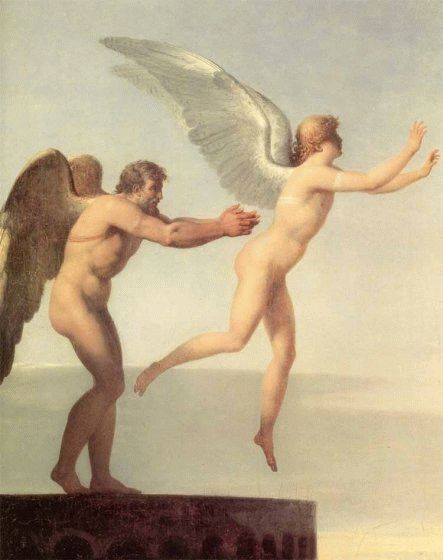
\includegraphics{images/Landon-IcarusandDaedalus.jpg}}
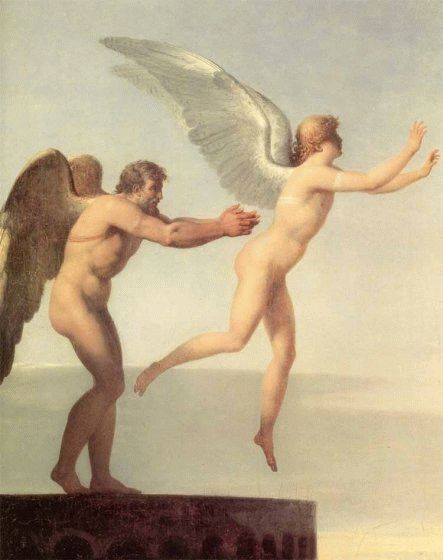
\includegraphics{images/Landon-IcarusandDaedalus.jpg}
\end{center}
\caption{Icarus and Daedelus}
\label{fig:icarus}
\end{figure}


\section{User Input}
The user input for Project Icarus consists of three groups of twenty 
infrared-emitting LEDs.  Each group of LEDs is strategically placed on the user to
determine arm position.  To do this, a group is placed on each wrist and one in
between the shoulders on the back.  This placement ensures that we can
accurately capture all the user movements that are needed to turn, glide, fall,
and flap.

The actual tracking devices are constructed of two pieces of Velcro stuck 
back-to-back.  This ensures that the user can easily don and remove them without
damaging the circuit (see figure~\ref{fig:circuit}) inside.  In order to wrap the tracking device
around an individual's wrist, stranded wire is soldered in between each LED.
This dramatically increases the flexibility of the circuit and reduces the
chance of having to re-solder any joint.  This is especially important since
the circuit is sandwiched between two pieces of Velcro that are stuck together
with adhesive.

\begin{figure}[h!t]
\begin{center}
\resizebox{\columnwidth}{!}{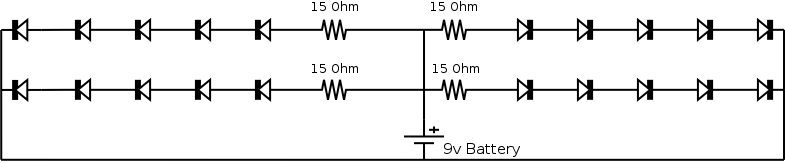
\includegraphics{images/circuit.png}}
%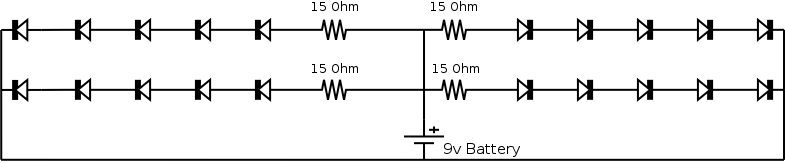
\includegraphics{images/circuit.png}
\end{center}
\caption{LED Circuit}
\label{fig:circuit}
\end{figure}

In order to capture the movement of the user, a common web camera (that does
not filter out infrared light) is placed on a tripod or other stable device
behind the user.  To ease in user tracking and block out all unwanted visible
light, a small piece of infrared pass filter material is placed between the
camera sensor and the lens.  The result is a black image except
for anything from an infrared source.  This means that any indoor lighting or
images from projectors will not show up.  This is important so that only the
LED tracking devices are seen from the camera.  The camera is then put slightly
out of focus to blur the LEDs in each group together to form one blob.  The
three light blobs are then used to calculate arm position (see section~\ref{sec:cv}).

Originally, no intrusive device was to be used for interaction: the idea was to
illuminate a person with an external infrared light source.  Unfortunately,
the size of source needed to illuminate an entire individual in a CAVE
environment is quite large and, ultimately, too expensive for the scope of this
particular project.  If more funding becomes available, this option will be
taken into greater consideration.

The light emitting circuit shown in figure~\ref{fig:circuit} requires \unit[9]{volts} and
approximately \unit[400]{mA} to operate.  Each light source includes a connection for a
standard \unit[9]{v} battery to satisfy the power needs.  A standard, rechargeable \unit[9]{v}
NiMH battery has about \unit[150]{mAh} of capacity but can go up to around \unit[625]{mAh} for
Alkaline.  To keep cost down, we try to use the rechargeable type whenever
possible.  Using rechargeable batteries, however, leads to less usable time
(about \unit[22]{minutes}), and the batteries need to be changed more often. 

\begin{figure}[h!t]
\begin{center}
\resizebox{3.0in}{!}{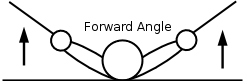
\includegraphics{images/wristforward.png}}
%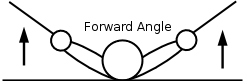
\includegraphics{images/wristforward.png}
\end{center}
\caption{Top view of input setup showing wrists too far forward}
\label{fig:wristforward}
\end{figure}

\begin{figure}[h!t]
\begin{center}
\resizebox{1.0in}{!}{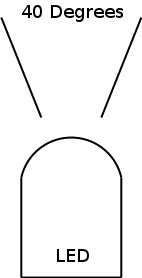
\includegraphics{images/led.png}}
%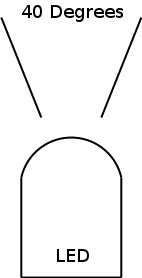
\includegraphics{images/led.png}
\end{center}
\caption{LED emission}
\label{fig:led}
\end{figure}

One issue that was not foreseen is the angles in which the user needs to hold
his or her arms.  If the user's wrist is far out of perpendicular to the camera
from a top view (see figure~\ref{fig:wristforward}), the light can disappear from the camera's
view.  This is due to a property of the LEDs and also the way in which they
are mounted.  The LEDs' emitted light is only visible when viewed from less
then approximately \unit[20]{degrees} off vertical (see figure~\ref{fig:led}).  The result of this
limitation is that when the user's arms come forward (away from camera) the
LEDs on the wrist are more likely to be out of this range and the stationary
camera is unable to detect the light.  Since the LEDs are mounted around the
wrist, the local wrist rotation is not as much of an issue as when the user
brings his or her wrists forward.  This is a limitation in the LEDs, so the
only solution would be adding LEDs facing in other directions.  Adding LEDs
would decrease the already short lifespan of the battery, thus, sufficient
instruction is given to the user to keep the lights relatively perpendicular to
the camera.

\section{Computational Perception}
\label{sec:cv}

Since our original idea of using gesture recognition on an IR-illuminated
person failed, we shifted to the method outlined above.  This greatly
simplified the computational techniques we had to employ.  The filtered image
(see figure~\ref{fig:filtered-image}) is surprisingly clean when we receive it
from the camera, so we didn't need to modify it much.  

\begin{figure}[h!t]
\begin{center}
\resizebox{\columnwidth}{!}{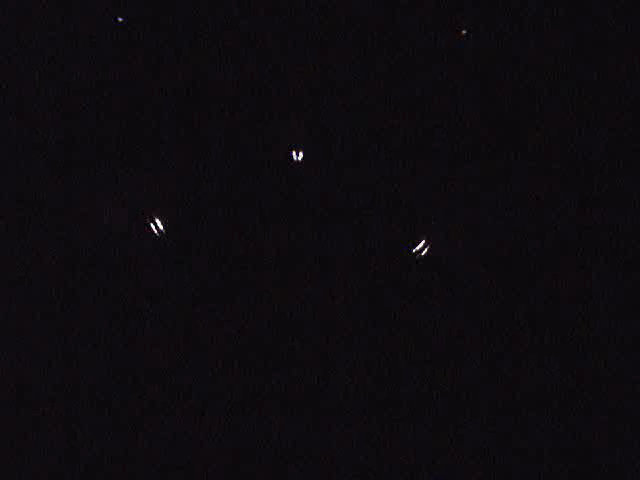
\includegraphics{images/filtered-image.png}}
%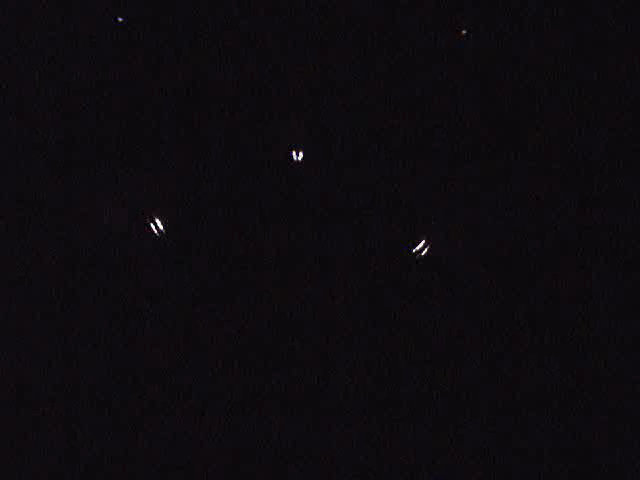
\includegraphics{images/filtered-image.png}
\end{center}
\caption{This IR-filtered frame from camera shows Ethan flapping his arms while in the C4 CAVE.  The two small white spots at the top of the image are the IR LEDs from the CAVE's tracking system.  The three larger blogs are the IR LEDs strapped to Ethan's wrists and back.}
\label{fig:filtered-image}
\end{figure}

\begin{figure}[h!t]
\begin{center}
\resizebox{\columnwidth}{!}{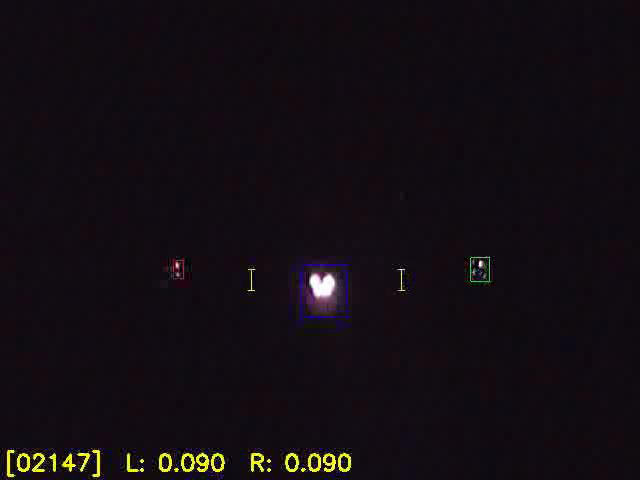
\includegraphics{images/processed-image.png}}
%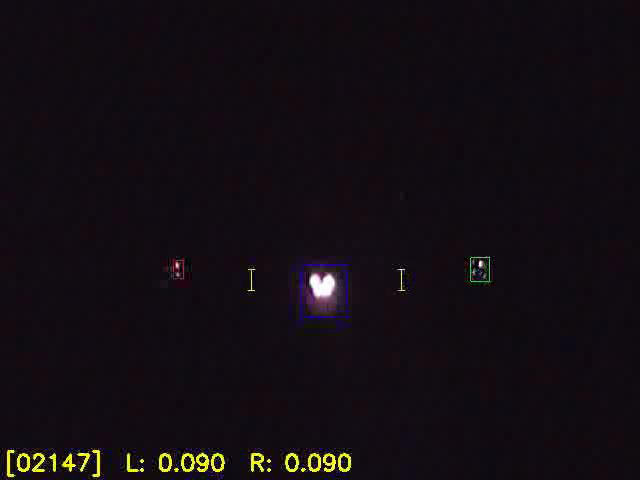
\includegraphics{images/processed-image.png}
\end{center}
\caption{The processed image highlights the left blob in red, the center blob in yellow, and the right blob in green.  The yellow lines show the vertical distance between the blobs.  The digits along the bottom of the image show the frame counter and the left and right vertical distances.}
\label{fig:processed-image}
\end{figure}


First, the image is converted from the RGB color space to greyscale.  Next, the
image is \emph{opened} by a six-pixel diameter disc-shaped structuring element.
The resulting image is \emph{dilated} twice with a $3\times3$ block-shaped
structuring element.

Next, the blobs are extracted from the image.  If the number of blobs is not
equal to three, the image is thrown out and we start again with the next frame
from the camera.  If three blobs are found, they are sorted by the $x$ position
of their centroids, from left to right.  Finally, the vertical distances
between the left and center blobs ($Y_l$) and right and center blobs ($Y_r$)
are calculated (see figure~\ref{fig:processed-image}).  These values are sent
via TCP socket to the simulator. 

\section{Flight Kinematics}

An important part of Project Icarus is turning the arm position information
from the camera into virtual flight.  During the development of Project Icarus
we experimented with two different flight models.  Our first attempt was a
force-based flight model.  In the end, we settled upon a velocity-based
approach that is not as realistic, but provides for a less frustrating
experience.  We used OPAL (Open Physics Abstraction Layer) as our physics
engine.  OPAL provides powerful features for simulating the application of
forces and torques to a rigid body.  

All of the interacting elements in the simulation (the ground plane, boxes, and
user bounding box) are represented by rectangular solids.  Each solid has a
number of properties that can be set such as density, size, center of gravity,
and material.  We used boxes that had a high density and materials that have no
friction coefficient.  The reason for not using friction is that the user would
have a tendency to tumble violently when contacting another solid.
Implementing a method for righting the user after tumbling would be useful,
however, we did not have time to do this and we do not think that the user
experience will suffer greatly.

Our first, force-based model was very simplistic and ad hoc.  We used three
forces applied to the user solid to achieve flight.  These forces are all
dependent on the normalized arm position.  The most important force for flight
is what we have termed the \emph{buoyant force}.  The buoyant force must increase when
the arms are extended, but not exceed the force of gravity to simulate soaring.
Also, the buoyant force must be greater than the force of gravity when the arms
are flapping to simulate powered flight.  Therefore, the buoyant force must be
proportional to the absolute value of the arm position and the derivative of
the arm position.  Another force that is important for the experience of flight
is a force that supplies a forward motion.  Not surprisingly, we chose to call
this force the \emph{forward force}.  In our case the forward force is constant unless
the user solid is in direct contact with another solid, in which case, the
forward force is zero.  Finally, in order to have controlled flight one must be
able to turn.  We calculated a \emph{turning torque} that operated about the vertical
axis and was proportional to the difference between the arm position from each
arm.

The force-based approach worked moderately well.  Unfortunately it suffered
from at least two problems that made control---and therefore the user experience---%
frustrating.  The first problem is that with a force-based approach it takes
work to overcome an opposing force.  For instance, gravity is always pulling
down on the user and it takes some flapping to overcome gravity and gain an
upward velocity.  No surprise there.  However, the inverse is also true.  If we
are applying an upward force by flapping our arms, then it takes time for
gravity to overcome our upward velocity and make us fall.  The other problem is
that the model does not account for any kind of centripetal force.  The very
simple combination of forward force and turning torque causes a phenomenon we
have dubbed \emph{hovercrafting}.  When hovercrafting, the user rotates about the
vertical axis to make a turn but the linear momentum of the user continues to
carry them in the same direction of travel until the constant forward force
restores forward flight (see figure~\ref{fig:hovercrafting}).  The combination
of these two problems made fine control of the user's position virtually
impossible when tested on a task such as flying between two closely spaced
blocks.

\begin{figure}[h!t]
\begin{center}
\resizebox{\columnwidth}{!}{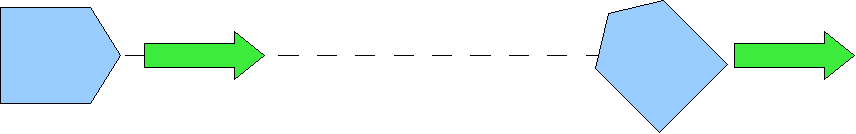
\includegraphics{images/hovercrafting.png}}
%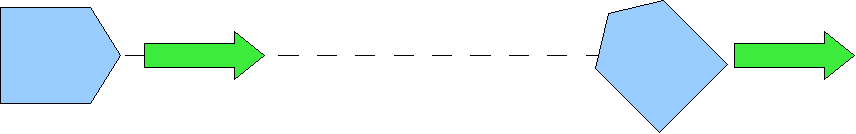
\includegraphics{images/hovercrafting.png}
\end{center}
\caption{Hovercrafting.}
\label{fig:hovercrafting}
\end{figure}

Our second, velocity-based model is actually just as simplistic and ad hoc as
the original force-based approach.  In fact, we used the same equations and
adjusted velocities directly instead of forces.  We replaced the buoyant force
with an upward velocity (figure~\ref{upward-velocity}), the forward force with
a forward velocity (figure~\ref{forward-velocity}), and the turning torque with
an angular velocity (figure~\ref{angular-velocity}).  After tweaking the
constant coefficients in the equations we were much more satisfied with our
flight model.  When flying through two closely-spaced boxes the user has much
tighter control over their own position.  The only artifact that seems very
unrealistic is the upward motion due to flapping.  As it is implemented it
feels a little too discontinuous.  This could probably be improved by using a
simple filter or hysteresis on the upward velocity.

\begin{figure}[h!t]
\begin{center}
%\resizebox{\columnwidth}{!}{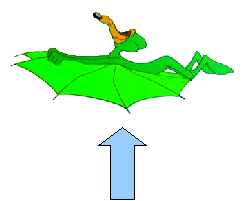
\includegraphics{images/upward-velocity.png}}
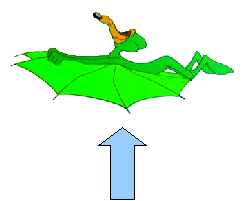
\includegraphics{images/upward-velocity.png}
\end{center}
\caption{The upward velocity is proportional to $\left|Y_l\right|+\left|Y_r\right|+\dot{Y}_l+\dot{Y}_r$.}
\label{fig:upward-velocity}
\end{figure}

\begin{figure}[h!t]
\begin{center}
%\resizebox{\columnwidth}{!}{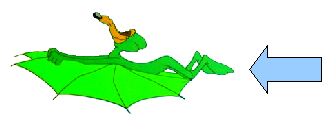
\includegraphics{images/forward-velocity.png}}
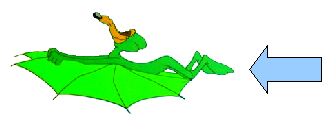
\includegraphics{images/forward-velocity.png}
\end{center}
\caption{The forward velocity is proportional to a constant.}
\label{fig:forward-velocity}
\end{figure}

\begin{figure}[h!t]
\begin{center}
%\resizebox{\columnwidth}{!}{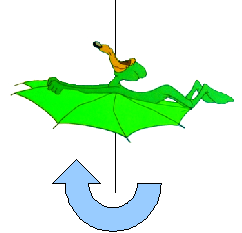
\includegraphics{images/angular-velocity.png}}
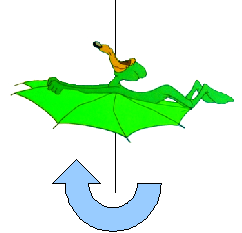
\includegraphics{images/angular-velocity.png}
\end{center}
\caption{The angular velocity is proportional to $Y_l - Y_r$.}
\label{fig:angular-velocity}
\end{figure}

\section{Graphics}
All the physics simulation in the world would still not make a flight
simulator.  In order for the user to become immersed in the experience they
must perceive the virtual.  Of course this is done with computer graphics.  Our
original goal in developing Project Icarus was to allow a person to experience
a simulation of human-powered flight in an immersive environment such as a CAVE
or a head-mounted display (HMD).  With this in mind we used VR Juggler as the
glue to bind the physics and graphics together into a portable, immersive
application.  VR Juggler allows us to, ``code once, experience everywhere.'' We
can use a laptop or desktop computer to debug or fly at home, as well as use a
CAVE or HMD for a truly immersive experience.

As mentioned above, we used OPAL for the physics layer.  For the graphics we
used OpenSceneGraph (OSG) which is an open source scene-graph library.  A
scene-graph greatly simplifies some aspects of graphics programming.
Scene-graphs take advantage of a tree-like structure to abstract concepts such
as grouping and transformation (see figure~\ref{fig:scenegraph}).  The graph
allows us to group graphical objects together and perform certain operations to
the whole group easily such as transforms, materials, switching, and lighting.
The graph also allows us to take advantage of one object in many instances,
such as using one box geometry to represent all boxes.  We did not take
advantage of many of these properties of the scene-graph in this work mainly
because they were not required and because it was a good excuse for the authors
to become familiar with this particular scene-graph implementation for another
project.

\begin{figure}[h!t]
\begin{center}
\resizebox{\columnwidth}{!}{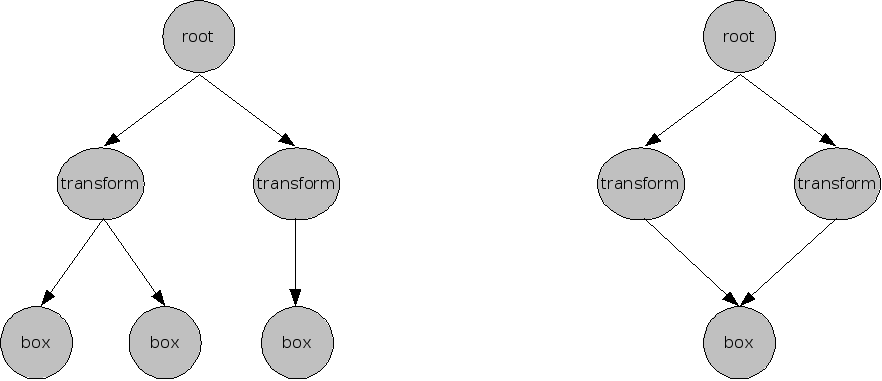
\includegraphics{images/scenegraph.png}}
%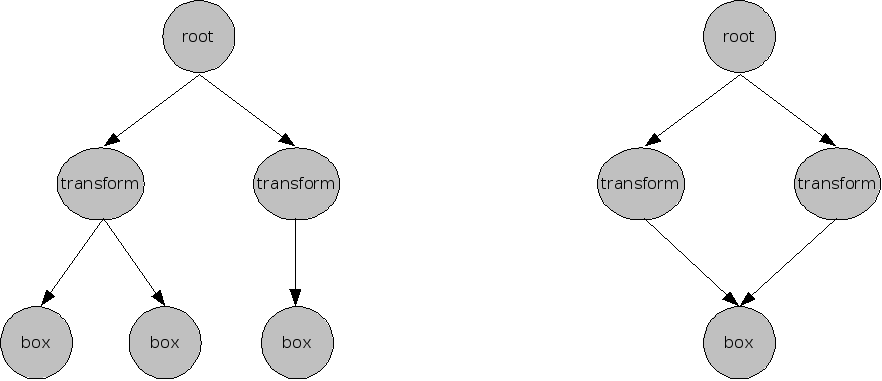
\includegraphics{images/scenegraph.png}
\end{center}
\caption{Two examples of scene-graphs.}
\label{fig:scenegraph}
\end{figure}

The environment that was created for Project Icarus is very simple.  Due to
limitations in the physics engine, the scene-graph library, and the authors'
skill, we represented all of the obstacles in the world as simple cubes on top
of a ground plane.  Very simple textures were created to give the world a look
similar to the 1980s movie \emph{Tron}.  Each box and the ground plane has a physical
representation as mentioned in preceding paragraphs.  Using OPAL gave us
collision detection and collision response for free.  Handling collisions is
something that is often done in the graphics.

\section{Conclusion}
We have a number of ideas for improvements to our project and ideas for future
work.  While our system seemed to hold up well in the environments in which we
tested it, it would be useful to have a variable threshold for the infrared
image.  This would help reduce the perception of ghost images and reflections
of the infrared light.  

We would also like to compile our program to run in the CAVE environment.
While we wrote our software with the CAVE in mind (using VR Juggler), we
haven't yet tested its performance live in the CAVEs.

We demonstrated our project to many of our classmates and were very pleased
by their reactions and by the performance of the system.  

\end{document}



